\pgfplotstablegetelem{\thepart}{[index]\columnIndex}\of{\cronograma}
\part{\pgfplotsretval}
\label{part:\thepart}
\frame{\partpage}


\begin{frame}[t]{Lógia de Programação - Resumo}
	
	\vspace{1em}
	
	\fontsize{14pt}{15}\selectfont{
		\begin{itemize}%[<+->]  
			\item \textbf{Lógica de Programação}:
			
			\begin{itemize}%[<+->]  
				\item Técnica de \underline{encadear} pensamentos para atingir determinado \underline{objetivo}.
				
				\item Necessária para desenvolver programas e sistemas, pois permite definir a \underline{sequência lógica} para a solução de um problema.
				
			\end{itemize}
			
			\item \textbf{Sequência Lógica}:
			
			\begin{itemize}%[<+->]  
				\item \underline{Passos} executados até se atingir o objetivo ou solução de um problema.
				
				\item Podem ser descritos como uma \underline{sequência de instruções}, que devem ser seguidas para se cumprir uma determinada tarefa.
				
			\end{itemize}			
			
		\end{itemize}
	}\par
	\vspace{1em}
	
\end{frame}



\begin{frame}[t]{Lógia de Programação - Instrução}
	
	
	\vspace{1em}
	
	\fontsize{16pt}{19}\selectfont{
		\begin{itemize}%[<+->]  
			\item \justifying Cada um dos {\color{red}passos}, cada uma das ações a tomar (obedecendo a sequência lógica) para ir resolvendo o problema, ou para ir executando a tarefa.
			
			\item \justifying Em computação, é a informação que indica a um computador uma {\color{red}operação} a executar. Ex: somar, subtrair.
			
			\item Uma só instrução não resolve problemas reais.
			
			\item Executar um {\color{red}conjunto de instruções}.
			
			\item Executar em {\color{red}uma sequência lógica}.		
			
		\end{itemize}
	}\par
	\vspace{1em}
	
\end{frame}



\begin{frame}[t]{Lógia de Programação - Algoritmo}
	
	%	\vspace{1em}
	
	\fontsize{16pt}{19}\selectfont{
		\begin{itemize}%[<+->]  
			\item {\color{red}Sequência finita de passos} que levam à execução de uma tarefa.
			
			\item Claro e preciso. Ex: somar dois números:
			
			\begin{itemize}%[<+->]  
				\item Escrever primeiro número no retângulo A
				\item Escrever segundo número no retângulo B
				\item Somar os números do retângulo A com o número do retângulo B e escrever o resultado no retângulo C.
				
			\end{itemize}		
			
			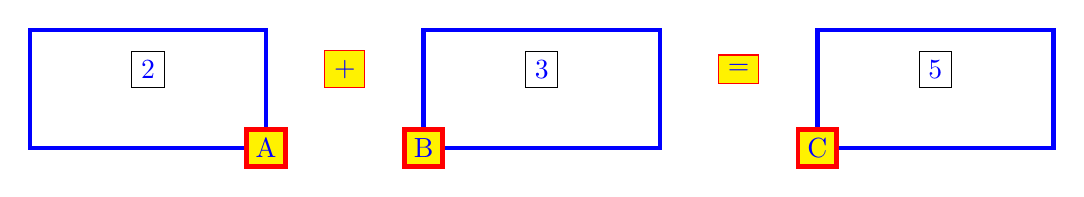
\begin{tikzpicture}
				
				%				\draw[blue, very thick] (0,0) rectangle (3,2);
				\draw[blue, ultra thick]  (0,3.5) rectangle (3,2) node[draw, color=red, fill=yellow, text=blue] {A};
				\draw[blue, ultra thick] (8,3.5) rectangle (5,2) node[draw, color=red, fill=yellow, text=blue] {B};
				\draw[blue, ultra thick] (13,3.5) rectangle (10,2) node[draw, color=red, fill=yellow, text=blue] {C};
				\draw (4,3) node[draw, color=red, fill=yellow, text=blue] {+};
				\draw (9,3) node[draw, color=red, fill=yellow, text=blue] {=};
				\draw (1.5,3) node[draw, text=blue] {2};
				\draw (6.5,3) node[draw, text=blue] {3};
				\draw (11.5,3) node[draw, text=blue] {5};
			\end{tikzpicture}
			
		\end{itemize}
	}\par
	\vspace{1em}
	
\end{frame}



\begin{frame}[t]{Lógia de Programação - Programa}
	
	\vspace{1em}
	
	\fontsize{16pt}{19}\selectfont{
		\begin{itemize}%[<+->]  
			\item {\color{red}Algoritmo} escrito em uma linguagem de computador (linguagem de programação).
			
			\item Interpretado e executado por um computador.
			
			\item Interpretação rigorosa, exata pelo computador -> escrita do algoritmo na linguagem de programação tem que seguir regras mais rigorosas.
			
		\end{itemize}
	}\par
	\vspace{1em}
	
\end{frame}




\begin{frame}[t]{Lógia de Programação - Plano}
	
	%	\vspace{1em}
	\fontsize{14pt}{19}\selectfont{
		Fases para desenvolver o algoritmo:
	}\par
	
	\fontsize{14pt}{19}\selectfont{
		\begin{itemize}%[<+->]  
			\item Determinar o problema, definí-lo (entender) bem.
			
			\item Dividir a solução nas três fases.
			
			
			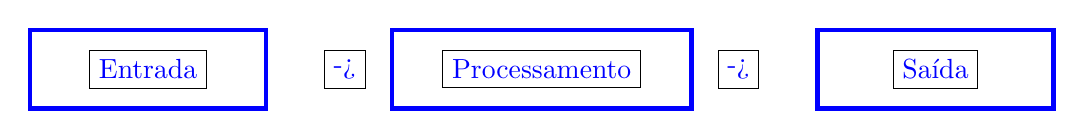
\begin{tikzpicture}
				
				%				\draw[blue, very thick] (0,0) rectangle (3,2);
				\draw[blue, ultra thick]  (0,3) rectangle (3,2);
				\draw[blue, ultra thick] (8.4,3) rectangle (4.6,2);
				\draw[blue, ultra thick] (13,3) rectangle (10,2);
				\draw (4,2.5) node[draw, text=blue] {->};
				\draw (9,2.5) node[draw, text=blue] {->};
				\draw (1.5,2.5) node[draw, text=blue] {Entrada};
				\draw (6.5,2.5) node[draw, text=blue] {Processamento};
				\draw (11.5,2.5) node[draw, text=blue] {Saída};
			\end{tikzpicture}
			
			
		\end{itemize}
	}\par
	\vspace{-0.5em}
	
	Exemplo:
	
	\fontsize{14pt}{19}\selectfont{
		\begin{itemize}%[<+->]  
			\item Problema: calcular a média de quatro números.
			
			\item Dados de entrada: os números N1, N2, N3 e N4.
			
			\item Processamento: somar os quatro números e dividir a soma por 4.
			
			\item Dado de saída: a média final
			
		\end{itemize}
	}\par
	\vspace{1em}
	
\end{frame}


\begin{frame}[t]{Vamos praticar}
	
	\vspace{1em}
	
	\fontsize{14pt}{19}\selectfont{
		Individualmente cada um escreve o seu algoritmo.
	}\par
	\vspace{1em}
	
	\centering
	
\includegraphics[scale=0.25]{imagens/fig-atencao-pessoas-estudando.png}
	
\end{frame}



\begin{frame}[t]{Lógia de Programação - Algoritmo}
	
	\vspace{1em}
	
	\fontsize{14pt}{19}\selectfont{
		\begin{itemize}%[<+->]  
			\item Início
			\item Ler o primeiro número
			\item Ler o segundo número
			\item ler o terceiro número
			\item Ler o quarto número
			\item Somar todos os números
			\item Dividir a soma por 4
			\item Mostrar o resultado da divisão
			\item Fim
			
		\end{itemize}
	}\par
	\vspace{1em}
	
\end{frame}




\begin{frame}[t]{Lógia de Programação - Python}
	
	\vspace{1em}
	\fontsize{14pt}{19}\selectfont{
		Escreva utilizando Python.
	}\par
	
	\vspace{1em}
	
	\centering
	
\includegraphics[scale=0.25]{imagens/fig-atencao-pessoas-estudando.png}
	
	
\end{frame}



\begin{frame}[t]{Exercício}
	
	\fontsize{12pt}{19}\selectfont{
		Escreva o algoritmo e programa.
		\begin{itemize}%[<+->]  
			
			\item \glsfirst{exercicio_013}: \glsdesc{exercicio_013}
			
			\vspace{1em}
			\centering
			
\includegraphics[scale=0.25]{imagens/fig-atencao-pessoas-estudando.png}
			
%			\item \glsfirst{exercicio_014}: \glsdesc{exercicio_014}
			
		\end{itemize}
	}\par
	\vspace{1em}
	
	
	
\end{frame}





\begin{frame}[t]{O que é uma função?}
	
	\vspace{1em}
	
	\fontsize{14pt}{25}\selectfont{
		\begin{itemize}%[<+->]  
			\item O conceito de função é um dos mais importantes na matemática.
			
			\item Em computação, uma função é uma sequência de instruções que computa um ou mais resultados que chamamos de parâmetros.
			
			\item Em aula utilizamos algumas funções já prontas do Python como o print() e input().
			
		\end{itemize}
	}\par
	\vspace{1em}
	
\end{frame}



\begin{frame}[t]{O que é uma função?}
	\fontsize{14pt}{15.2}\selectfont{
		
		O Python permite definirmos funções. A sintaxe é muito parecida	com a da matemática. Para definirmos uma função no Python utilizamos o comando def:	
		\vspace{1em}
		
		\begin{beamercolorbox}[wd=\textwidth]{warning}
			def somar(primeiroNumero, segundoNumero):\\
			\hspace{2em}return primeiroNumero + segundoNumero\\
			\vspace{1em}
			print('total da soma: {}'.format(somar(11,20)))
		\end{beamercolorbox}
		
	}\par
	\vspace{1em}
	
\end{frame}


\begin{frame}[t]{Exemplo de função}
	
	\vspace{3em}
	\lstinputlisting[style=CBruno,caption=Exemplo de Código para criação de função em python]{outros/codigos/python/codigo_001_somar.py}
	
	\vspace{3em}
	\lstinputlisting[style=CBruno,caption=Exemplo de Código para criação de dois casos de testes para a função somar.]{outros/codigos/python/test_codigo_001_somar.py}
	
\end{frame}


\begin{frame}[t]{Pytest}
	
	\vspace{3em}
	\begin{beamercolorbox}[wd=\textwidth]{warning}
		pip install pytest\\
		\vspace{1em}
		pip install pytest-cov\\
		\vspace{1em}
		python -m pytest --cov\\
		\vspace{1em}
		python -m pytest --cov -q test\_filename.py\\
		\vspace{1em}
		coverage html \&\& open htmlcov/index.html
	\end{beamercolorbox}
	\vspace{1em}
	*obs: são dois traços antes da palavra cov.\\
	*obs: o nome do arquivo que contém os testes deve iniciar com prefíxo test\_*, em que o asterisco deve ser substituído pelo "nome do código" que será testado. Exemplo: arquivo test\_codigo\_001\_somar.py utilizado para testar o arquivo codigo\_001\_somar.py
	
	\vspace{3em}
	\url{https://docs.pytest.org/en/7.1.x/contents.html}
	
\end{frame}


\begin{frame}[t]{Pytest}
	
	\vspace{3em}
	\centering
	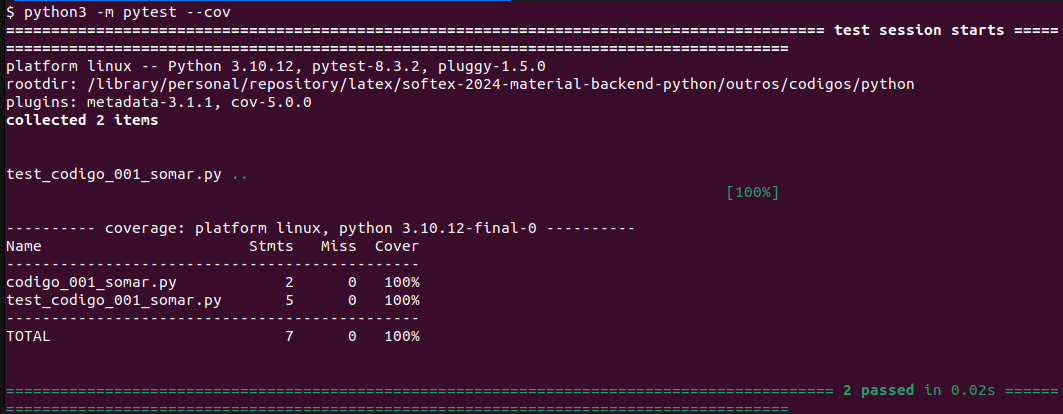
\includegraphics[scale=0.35]{imagens/fig-test-result-sample.png}
	
\end{frame}


\begin{frame}[t]{Pytest}
	
	\centering
	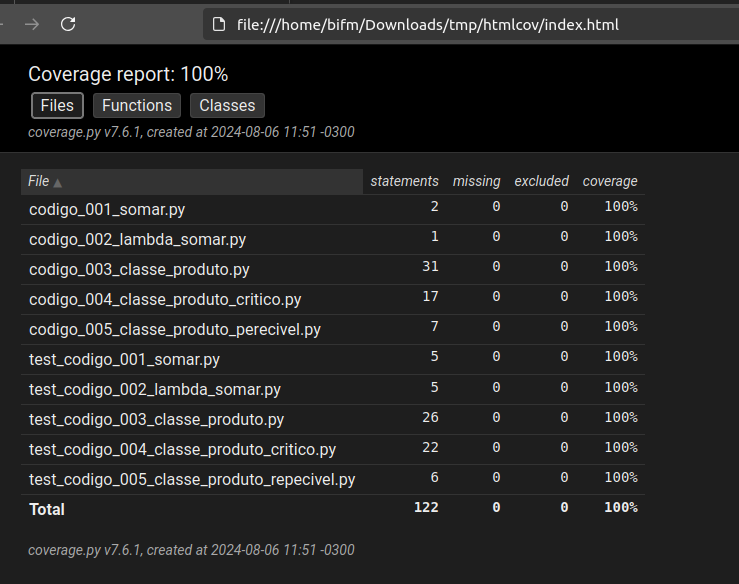
\includegraphics[scale=0.32]{imagens/fig-exemplo-resultado-teste-com-coverage-html.png}
	
\end{frame}




\begin{frame}[t]{Exercício}
	
	\fontsize{12pt}{19}\selectfont{
		Escreva o programa.
		\begin{itemize}%[<+->]  
			
			\item \glsfirst{exercicio_025}: \glsdesc{exercicio_025}
			
			\vspace{1em}
			\centering
			
\includegraphics[scale=0.25]{imagens/fig-atencao-pessoas-estudando.png}
			
			
			
		\end{itemize}
	}\par
	\vspace{1em}
	
\end{frame}



\begin{frame}[t]{Exercício}
	
	\fontsize{12pt}{19}\selectfont{
		Escreva o programa.
		\begin{itemize}%[<+->]  
			
			\item \glsfirst{exercicio_026}: \glsdesc{exercicio_026}
			
			\vspace{1em}
			\centering
			
\includegraphics[scale=0.25]{imagens/fig-atencao-pessoas-estudando.png}
			
			
			
		\end{itemize}
	}\par
	\vspace{1em}
	
\end{frame}



\begin{frame}[t]{Exemplos com função input()}	
	
	\vspace{3em}
	\lstinputlisting[style=CBruno,caption=Código para criação de função com input()]{outros/codigos/python/codigo_008_input.py}
	
\end{frame}

\begin{frame}[t]{Pytest}
		
	\lstinputlisting[style=CBruno,caption=Teste para funções criadas com input()]{outros/codigos/python/test_codigo_008_input.py}
	
\end{frame}

\begin{frame}[t]{Pytest}

	\vspace{1em}
	\centering
	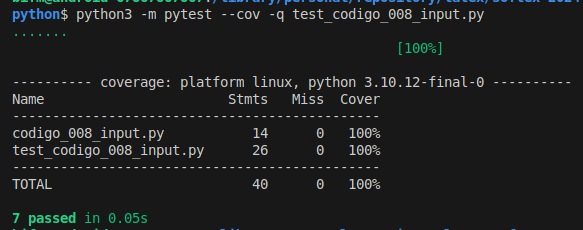
\includegraphics[scale=0.65]{imagens/fig-test-result-input.png}
	
\end{frame}



\begin{frame}[t]{Exemplos com função print()}	
	
	\vspace{3em}
	\lstinputlisting[style=CBruno,caption=Código para criação de função com print()]{outros/codigos/python/codigo_009_print.py}
	
\end{frame}

\begin{frame}[t]{Pytest}
	\vspace{-1em}
	\lstinputlisting[style=CBruno,caption=Teste para funções criadas com print()]{outros/codigos/python/test_codigo_009_print.py}
	
\end{frame}

\begin{frame}[t]{Pytest}
	
	\vspace{1em}
	\centering
	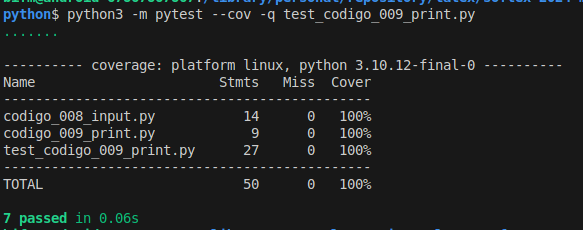
\includegraphics[scale=0.65]{imagens/fig-test-result-print.png}
	
\end{frame}






\begin{frame}[t]{Exercícios}
	
	\fontsize{12pt}{19}\selectfont{
		\begin{itemize}%[<+->]  
			
			
			\item \glsfirst{exercicio_015}: \glsdesc{exercicio_015}
			
			\item \glsfirst{exercicio_016}: \glsdesc{exercicio_016}
			
		\end{itemize}
	}\par
	\vspace{1em}
	
\end{frame}


\begin{frame}[t]{Exemplo de função anônima (lambda)}
	
	\fontsize{12pt}{15.2}\selectfont{
		
		Funções lambda são uma ferramenta poderosa e versátil na programação Python, que permite criar funções anônimas de forma simples e rápida.
		
		\vspace{1em}
		Uma função lambda é criada usando a palavra-chave lambda, seguida de um ou mais argumentos, e uma expressão.	
		\vspace{1em}
		
		Argumentos são os dados de entrada que esta função irá receber expressão é o código que será executado quando a função lambda for chamada.
		
		\vspace{1em}
		Sua sintaxe básica é a seguinte:
		
		\vspace{1em}
		\begin{beamercolorbox}[wd=\textwidth]{warning}
			lambda {argumentos}: {expressão}
		\end{beamercolorbox}
		
		
	}\par
	\vspace{1em}
	
	
\end{frame}



\begin{frame}[t]{Exemplos de funções anônimas (lambda)}	
	
	\vspace{3em}
	\lstinputlisting[style=CBruno,caption=Exemplo de Código para criação de função anônima em python]{outros/codigos/python/codigo_002_lambda_somar.py}
	
\end{frame}




\begin{frame}[t]{Pytest}
	
	
	\lstinputlisting[style=CBruno,caption=Exemplo de Código para testar função anônima em python]{outros/codigos/python/test_codigo_002_lambda_somar.py}
	
	\vspace{1em}
	\centering
	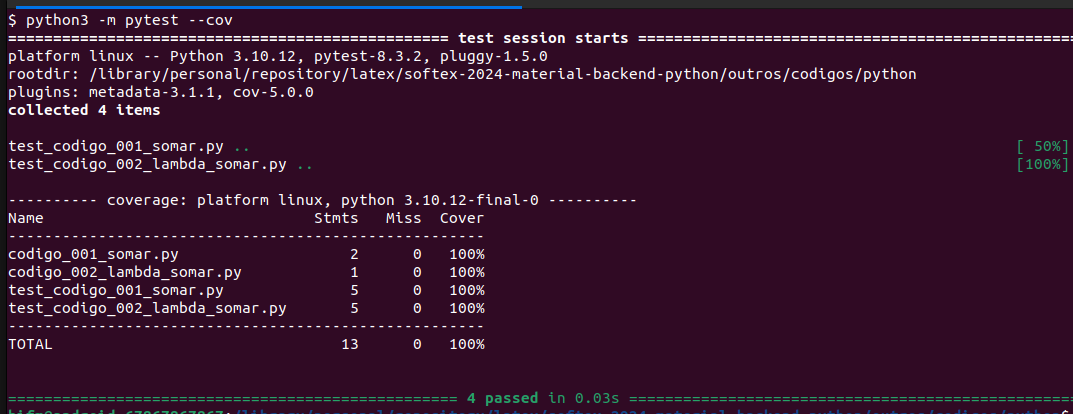
\includegraphics[scale=0.25]{imagens/fig-result-test-lambda-somar.png}
	
\end{frame}




\begin{frame}[t]{Exercícios}
	
	\fontsize{12pt}{19}\selectfont{
		\begin{itemize}%[<+->]  
			
			\item \glsfirst{exercicio_017}: \glsdesc{exercicio_017}
			
			
		\end{itemize}
	}\par
	\vspace{1em}
	
\end{frame}







